В этом параграфе мы будем работать со следующими степенными рядами:
\begin{equation}\label{plain-series}
\sum\limits_{n=0}^\infty c_n z^n
\end{equation}
\begin{equation}\label{absolute-series}
\sum\limits_{n=0}^\infty |c_n z^n|
\end{equation}

\begin{theorem}[Абеля]\label{Abel}
Пусть ряд \ref{plain-series} сходится для некоторого \(\widetilde{z} \neq 0\), тогда 
\begin{enumerate}
    \item \(\forall z\,\left(|z| < |\widetilde{z}|\: \Rightarrow \text{ ряд \ref{plain-series} сходится абсоютно} \right)\) 
    \item \(\forall r\, \left(0 < r < |\widetilde{z}|\: \Rightarrow \text{ ряд \ref{plain-series} сходится равномерно по } z \text{ в круге } \overline{B}_r(0) =: K \right)\)
\end{enumerate}
\end{theorem}

\begin{proof}
    Докажем сначала пункт 2: т. к. \(\sum\limits_{n=0}^\infty c_n \widetilde{z}^n\) сходится, то \(c_n \widetilde{z}^n \xrightarrow[n \to \infty]{}0\). Значит, \(\exists M > 0\, \forall n \left(|c_n \widetilde{z}^n| \leqslant M \right)\). Тогда \(\forall z \in K\) верно \(|c_n z^n| = |c_n \widetilde{z}^n| \cdot \left|\frac{z}{\widetilde{z}} \right|^n \leqslant M \left| \frac{z}{\widetilde{z}} \right|^n \). Так как ряд \(\sum\limits_{n=0}^\infty M \left|\frac{z}{\widetilde{z}} \right|^n\) сходится как геом. прогрессия со знаменателем меньше 1, то по признаку Вейерштрасса на \(K\) сходится и ряд \ref{absolute-series}, а значит и ряд \ref{plain-series}. \\
    Для док-ва пункта 1 достаточно выбрать любое \(r\), подходящее под условия \(|z| \leqslant r < |\widetilde{z}|\) и применить уже доказанный пункт 2.
\end{proof}

\begin{definition}[радиус сходимости] \(\crad := \sup \left\{|z|:\: \text{ряд \ref{plain-series} сходится при этом } z \right\}\).
\end{definition}

\begin{corollary}
\begin{itemize}
    \item \(\forall z \left(|z| < \crad \: \Rightarrow \text{ ряд \ref{plain-series} сход. абс.} \right) \)
    \item \(\forall z \left(|z| > \crad\: \Rightarrow \text{ряд \ref{plain-series} расходится}\right) \)
\end{itemize}
\end{corollary}

\begin{unnecessary}
    \begin{note}[формула Коши--Адамара]
    Из курса мат. анализа известно, что 
    \[R_{\text{сх}} = \dfrac{1}{\overline{\lim\limits_{n \to \infty}} \left(|c_n|^{1/n} \right)}\]
    \end{note}
\end{unnecessary}

\begin{definition}[круг сходимости]
    \textit{Кругом сходимости} ряда \ref{plain-series} называется \(K = \left\{z:\: |z| < \crad \right\}\).
\end{definition}

\begin{corollary}
    В круге сходимости ряда его сумма является непрерывной функцией.
\end{corollary}

\begin{theorem}[о дифференцируемости суммы степенного ряда]
    Пусть ряд \ref{plain-series} сходится в круге \(K = \left\{z:\: |z| < R \right\}\) для какого-то \(R > 0\) к сумме \(S(z)\), тогда
    \begin{enumerate}
        \item ряд \(\sum\limits_{n=1}^\infty n c_n z^{n-1}\) сходится в круге \(K\)
        \item \(\widehat{S}(z):=\sum\limits_{n=1}^\infty n c_n z^{n-1} = S'(z)\)
    \end{enumerate}
\end{theorem}

\begin{proof}
Для начала докажем пункт 1. Для этого зафкиксируем \(z\ in K\). Выберем \(\widetilde{z}\), такой, что \(|z| < |\widetilde{z}| < R\), тогда
\[|n c_n z^{n-1}| = |c_n \widetilde{z}^n| \cdot \frac{n}{|\widetilde{z}|} \cdot \left| \frac{z}{\widetilde{z}} \right|^{n-1} =: |c_n \widetilde{z}^n| \cdot A_n\]
Так как \(A_n \xrightarrow[n \to \infty]{} 0\), то начиная с некоторо номера \(n\) выполняется следущее неравенство:\\
\(|n c_n z^{n-1}| \leqslant |c_n \widetilde{z}^n|\). Так как ряд \ref{plain-series} сходится при \(\widetilde{z}\), то сходится и ряд \(\sum\limits_{n=1}^\infty |n c_n z^{n-1}|\) и тем более ряд \(\sum\limits_{n=1}^\infty n c_n z^{n-1}\).

Теперь будем доказывать пункт 2. Для этого зафиксируем \(z \in K\) И число \(\varepsilon > 0\). Зафиксируем \(r\) такое, что \(|z| < r < R\). В силу сходимости ряда \(\sum\limits_{n=1}^\infty n |c_n|r^{n-1}\) существует \(N\) такое, что \(\sum\limits_{n=N+1}^\infty n |c_n|r^{n-1} < \infty\). Зафиксируем такое \(N\). Будем выбирать \(\Delta z\) как \(|z +\Delta z| < r \wedge |\Delta z| \neq 0\). Рассмотрим
\[A(\Delta z) = \left|\frac{S(z + \Delta z) - S(z)}{\Delta z} - \widehat{S}(z) \right| =: \left|B(\Delta z) - \widehat{S}(z) \right|\]
При этом 
\begin{multline*}
B(\Delta z) = \frac{1}{\Delta z} \sum\limits_{n=1}^\infty c_n \left[(z + \Delta z)^n - z^n \right] = \biggr/a^n - b^n = (a-b)(a^{n-1} + a^{n-2}b + \ldots + b^{n-1}) \biggr/ =\\
=\sum\limits_{n=1}^\infty c_n \left[(z + \Delta z)^{n-1} + (z + \Delta z)^{n-2}z + \ldots + z^{n-1} \right]
\end{multline*}
Вопсользуемся неравенством треугольника и представим \(A(\Delta z)\) в виде трёх частей:
\begin{align*}
     A(\Delta z) \leqslant \left| \sum\limits_{n=1}^N c_n \left( \left[(z + \Delta z)^{n-1} + (z + \Delta z)^{n-2}z + \ldots + z^{n-1} \right] - nz^{n-1} \right) \right| +\\
     + \left| \sum\limits_{n=N+1}^\infty c_n \left[(z + \Delta z)^{n-1} + (z + \Delta z)^{n-2}z + \ldots + z^{n-1} \right] \right| + \\
     + \left| \sum\limits_{n=N+1}^\infty n c_n z^{n-1} \right| =: A_1(\Delta z) + A_2(\Delta z) + A_3(\Delta z)
\end{align*}
\(A_1(\Delta z)\) --- модуль многочлена от \(\Delta z\), при этом \(A_1(0) = 0\), значит
\[\exists \delta > 0\,\forall \Delta z \left(|\Delta z| < \delta \rightarrow A_1(\Delta z) < \varepsilon \right)\] \\
Также \(|z + \Delta z| < r\), а значит в силу выбора \(N\)
\[A_2(\Delta z) \leqslant \sum\limits_{n=N+1}^\infty |c_n| \cdot \left[|z + \Delta z|^{n-1} + \ldots + |z|^{n-1} \right] \leqslant \sum\limits_{n=N+1}^\infty n |c_n| \cdot r^{n-1} < \varepsilon\]
При этом также в силу выбора \(N\)
\[A_3(\Delta z) \leqslant \sum\limits_{n=N+1}^\infty n|c_n|r^{n-1} < \varepsilon\]
Значит, при \(|z + \Delta z| < r\) и \(0 < |\Delta z| < \delta\) имеем \(A(\Delta z) < 3 \varepsilon\). Значит, в силу произвольности выбора \(\varepsilon > 0\) получаем, что \(\widehat{S}(z) = S'(z)\).
\end{proof}

\begin{corollary}
    Т. к. функция \(\widehat{S}(z)\) непрерывна на \(K\), то \(S(z)\) регулярна на \(K\).
\end{corollary}

\begin{corollary}
    Применяя аналогичные рассуждения к ряду \(\widehat{S}(z)\) получаем, что \(S(z)\) дифференцируема бесконечное количество раз на круге \(K\) и при этом \(S^{(n)}(0) = n! c_n\), то есть \\
    \(S(z) = \sum\limits_{n=0}^\infty \dfrac{S^{(n)}(0)}{n!}z^n \), а значит, ряд \ref{plain-series} является рядом Тейлора для своей суммы.
\end{corollary}

% \begin{figure}[H]
%     \centering
%     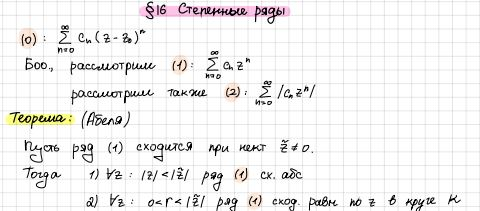
\includegraphics[width=350pt]{images/16_1.JPG}
% \end{figure}

% \begin{figure}[H]
%     \centering
%     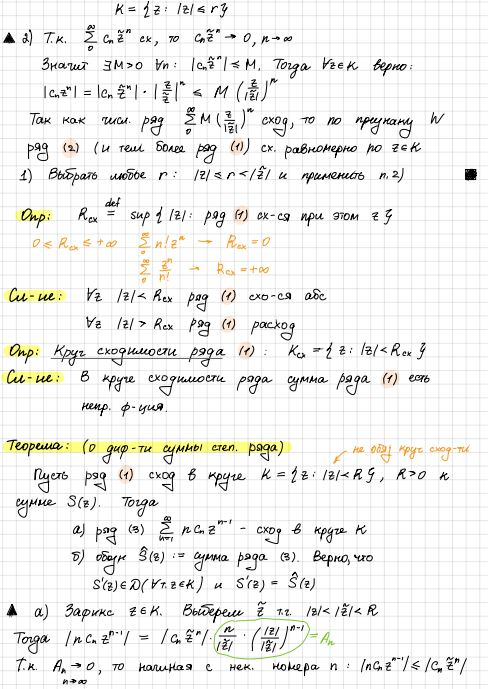
\includegraphics[width=350pt]{images/16_2.JPG}
% \end{figure}

% \begin{figure}[H]
%     \centering
%     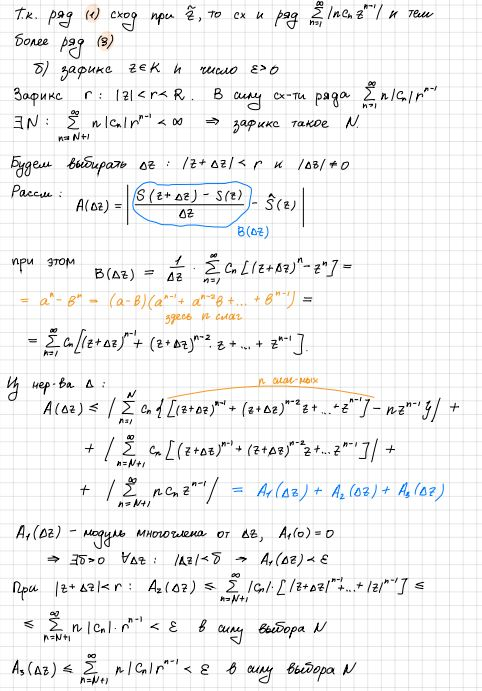
\includegraphics[width=350pt]{images/16_3.JPG}
% \end{figure}

% \begin{figure}[H]
%     \centering
%     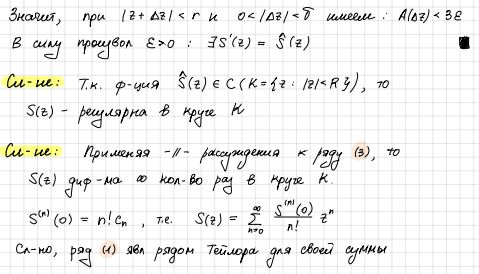
\includegraphics[width=350pt]{images/16_4.JPG}
% \end{figure}
